\documentclass[12pt]{article}

% ---------- Packages ----------
\usepackage[margin=1in]{geometry}
\usepackage{amsmath, amssymb}
\usepackage{graphicx}
\usepackage{booktabs}
\usepackage{caption}
\usepackage{setspace}
\usepackage{authblk}
\usepackage[round]{natbib}
\usepackage[hidelinks]{hyperref}
\usepackage{float}

\onehalfspacing
\captionsetup{font=small}

\title{Smoke and Strife: Fire Exposure and Social Conflict in Indonesia}
\author{Hariaksha Gunda\thanks{Email: \href{mailto:hgunda@crimson.ua.edu}{hgunda@crimson.ua.edu}. Code is available at \url{https://github.com/Hariaksha/smoke-and-strife}. This is a ten-page version of a longer working paper, which reports the full set of robustness checks. All errors are my own.}}
\affil{The University of Alabama}
\date{Writing sample, \today}

\begin{document}

\maketitle

\begin{abstract}
\noindent Seasonal land and forest fires blanket much of Indonesia in haze each year. Using fire activity upwind of each of 481 districts, which changes a district's smoke exposure through the wind rather than through local conditions, I find that upwind fire reduces monthly conflict events where conflict is common, by a similar small percentage everywhere. The result is robust to excluding the district's own fires, controlling for local weather, and a placebo using next month's fire. Two tests point to two channels. Protests fall with smoke from fires in other provinces, consistent with a direct effect of smoke. Events carried out by security forces fall about five times as much in proportional terms, and significantly only with fires in the district's own province, whose fire task forces the same forces lead, consistent with diversion of state capacity. Fatal events fall more than other events, which argues against a reporting explanation.

\medskip
\noindent\textbf{JEL codes:} Q53, Q54, D74, H56 \quad \textbf{Keywords:} air pollution, wildfire, conflict, Indonesia, state capacity
\end{abstract}

\section{Introduction}

A large literature links climate variation to conflict, typically through slow-moving channels such as income shocks and resource scarcity \citep{hsiang2013quantifying, burkehsiangmiguel2015}. Indonesia offers a different kind of shock. Each dry season, land-clearing fires, intensified by El Ni\~{n}o, produce haze across much of the archipelago. Its effect on conflict is not obvious in advance. Air pollution raises individual violent crime \citep{herrnstadt2021, burkhardt2019}, which predicts more conflict. But haze may also keep people indoors and draw police and military units into firefighting, which predicts less of the collective and state-led contention recorded in conflict data.

Local fires are a poor measure of exposure, because the land disputes and weak governance that drive conflict may also drive land-clearing fires. I therefore exploit the physics of smoke transport. For each district and month, I measure the fire radiative power (FRP) of fires within 300\,km and within $45^{\circ}$ of the direction the wind blows from, whose smoke the wind would carry toward the district. Conditional on district and year-month fixed effects, this upwind fire changes a district's smoke exposure but is plausibly unrelated to its own political and economic shocks. I build the measure for 481 districts, linking NASA VIIRS fire detections, ERA5 wind fields, and ACLED conflict events in a panel of 60,125 district-months from 2015 to 2025.

In districts where conflict occurs in at least 30\% of months, a one-log-point increase in upwind FRP reduces conflict events by 0.026 per district-month ($p=0.002$), 1.9\% of the mean. Across all districts the estimate is small and insignificant, but the two results are consistent: in proportional terms the effect is about the same in all districts, and it is measurable in event counts only where conflict is frequent. The estimate survives a placebo using next month's fire, the exclusion of fires inside the district, and controls for local weather.

The pattern of declines points to two channels. Events carried out by state forces fall about five times as much as peaceful protests in proportional terms, fatal events fall more than other events, and imprecisely recorded events do not fall, which argues against a reporting explanation. Because Indonesia organizes its fire task forces by province, I also separate fires in a district's own province, which draw on its security forces, from fires in other provinces, which reach it only as smoke. Protests fall with other-province fire, pointing to smoke itself; state violence falls significantly only with same-province fire, consistent with the diversion of security forces to fire response. The paper thus finds the opposite sign to the pollution-crime literature \citep{herrnstadt2021, bondyrothsager2020, burkhardt2019} for collective and state-led contention, and brings district-level evidence to the debate over whether disasters raise or lower conflict \citep{nelrigharts2008, slettebak2012, woodwright2016}.

\section{Setting and Data}
\label{sec:data}

Smoke from Indonesian fires is a severe pollution shock: the 1997 fires caused an estimated 15,600 child and infant deaths \citep{jayachandran2009}. Fire response draws directly on the security forces. Presidential instructions issued in 2015 and 2020 direct the armed forces and national police to deploy personnel to fight fires and patrol fire-prone areas, and under the 2020 instruction the provincial military commander and police chief serve as deputy commanders of each province's fire task force \citep{inpres11_2015, inpres3_2020}.

Fire detections come from the VIIRS active fire product (375\,m), restricted to high- and nominal-confidence vegetation fires, each with its fire radiative power. Monthly wind, precipitation, and temperature come from ERA5 \citep{hersbach2023era5}. Conflict events come from ACLED, January 2015 to June 2025; I assign each event to the GADM district polygon containing its coordinates, since ACLED's district names merge cities with surrounding regencies. The panel crosses the 481 districts with any event with 125 months. Conflict is rare: 82.9\% of district-months record no event.

\section{Empirical Strategy}
\label{sec:empirical}

\paragraph{The upwind measure.} For district $d$ in month $t$, upwind fire activity is
\[
Z_{dt} = \sum_{f \in \mathcal{U}_{dt}} \text{FRP}_f,
\]
where $\mathcal{U}_{dt}$ contains the fire detections in month $t$ that lie within 300\,km of the district's centroid and within $\pm 45^{\circ}$ of the direction its wind blows from. These are fires whose smoke the wind would carry toward the district. It enters regressions as $\text{logZ}_{dt} = \log(1+Z_{dt})$.

\paragraph{Reduced form.} The specification is
\begin{equation}
y_{dt} = \alpha_d + \gamma_t + \pi_0\, \text{logZ}_{dt} + \pi_1\, \text{logZ}_{d,t-1} + \varepsilon_{dt},
\label{eq:rf}
\end{equation}
where $y_{dt}$ is a conflict count, $\alpha_d$ are district fixed effects, and $\gamma_t$ are year-month fixed effects, which absorb national shocks and seasonality. The lag allows smoke and its consequences to persist into the next month. Standard errors are clustered by province (34 clusters). The coefficient of interest, $\pi_0$, is the effect of wind-borne exposure to upwind fire on conflict. It is identified if, after removing district and year-month means, the month-to-month variation in upwind fire created by the wind is unrelated to the district's own conflict shocks. Because the wind direction that defines ``upwind'' changes from month to month, the measure picks up different fires in different months for the same district.

\paragraph{Why not instrument local fire?} Upwind fire strongly predicts local fire (effective $F = 81.3$; \citealp{montielolea2013}), but an IV of conflict on local fire would require upwind fire to matter only through local fire, which fails if smoke changes behavior, the mechanism of interest. The reduced form is therefore the main evidence. The main threats are regional shocks, such as droughts, that raise both upwind fire and conflict; fires inside the district, which the upwind cone partly includes; and haze-driven changes in conflict reporting. I address each below.

\section{Results}
\label{sec:results}

Table~\ref{tab:rf} reports the reduced form in the full panel and in the 85 districts with conflict in at least 30\% of months. In the full panel, all coefficients are negative but small and insignificant. In the conflict-active districts, upwind fire reduces all events by 0.026 per log point ($p=0.002$; Anderson--Rubin $p=0.012$), and the decline in political violence comes from riots and violence against civilians.

\begin{table}[H]
\centering
\caption{Reduced form: effect of upwind fire on monthly conflict events}
\label{tab:rf}
\footnotesize
\begin{tabular}{lcccc}
\toprule
 & All events & Political violence & Riots and VAC & VAC \\
\midrule
\multicolumn{5}{l}{\emph{Full panel (481 districts, 60,125 district-months)}} \\
$\text{logZ}_{dt}$ & $-0.0024$ & $-0.0008$ & $-0.0008$ & $-0.0007$ \\
 & (0.0020) & (0.0006) & (0.0006) & (0.0005) \\
Mean of outcome & 0.360 & 0.059 & & \\
\addlinespace
\multicolumn{5}{l}{\emph{Conflict-active districts (85 districts, 10,625 district-months)}} \\
$\text{logZ}_{dt}$ & $-0.0261^{***}$ & $-0.0072^{*}$ & $-0.0079^{**}$ & $-0.0055^{*}$ \\
 & (0.0078) & (0.0039) & (0.0037) & (0.0029) \\
Mean of outcome & 1.398 & 0.220 & 0.167 & 0.072 \\
Anderson--Rubin $p$ & 0.012 & 0.164 & 0.066 & 0.024 \\
\bottomrule
\end{tabular}
\begin{minipage}{0.95\textwidth}
\vspace{4pt}
\footnotesize \emph{Notes:} Coefficient on contemporaneous log upwind FRP from Eq.~\eqref{eq:rf}, which also includes its one-month lag and district and year-month fixed effects. Standard errors clustered by province (34 clusters) in parentheses. VAC is violence against civilians. Conflict-active districts record at least one event in at least 30\% of months. The Anderson--Rubin test is the joint test that both instrument coefficients are zero, for the IV of local fire on the outcome. $^{***}p<0.01$, $^{**}p<0.05$, $^{*}p<0.1$.
\end{minipage}
\end{table}

Because the 30\% cutoff is measured over the estimation window, I also group districts by their number of months with conflict in 2015--2017 and estimate on 2018--2025. The effect is near zero in districts with no prior conflict ($+0.003$) and largest in the 41 districts with six or more months of it ($-0.040$, $p=0.037$). A Poisson version shows no gradient in proportional terms (about $-1\%$ per log point everywhere; interaction $p=0.60$): upwind fire reduces conflict by a similar small percentage in all districts, which is detectable only where conflict is common (Figure~\ref{fig:propensity}).

\begin{figure}[H]
\centering
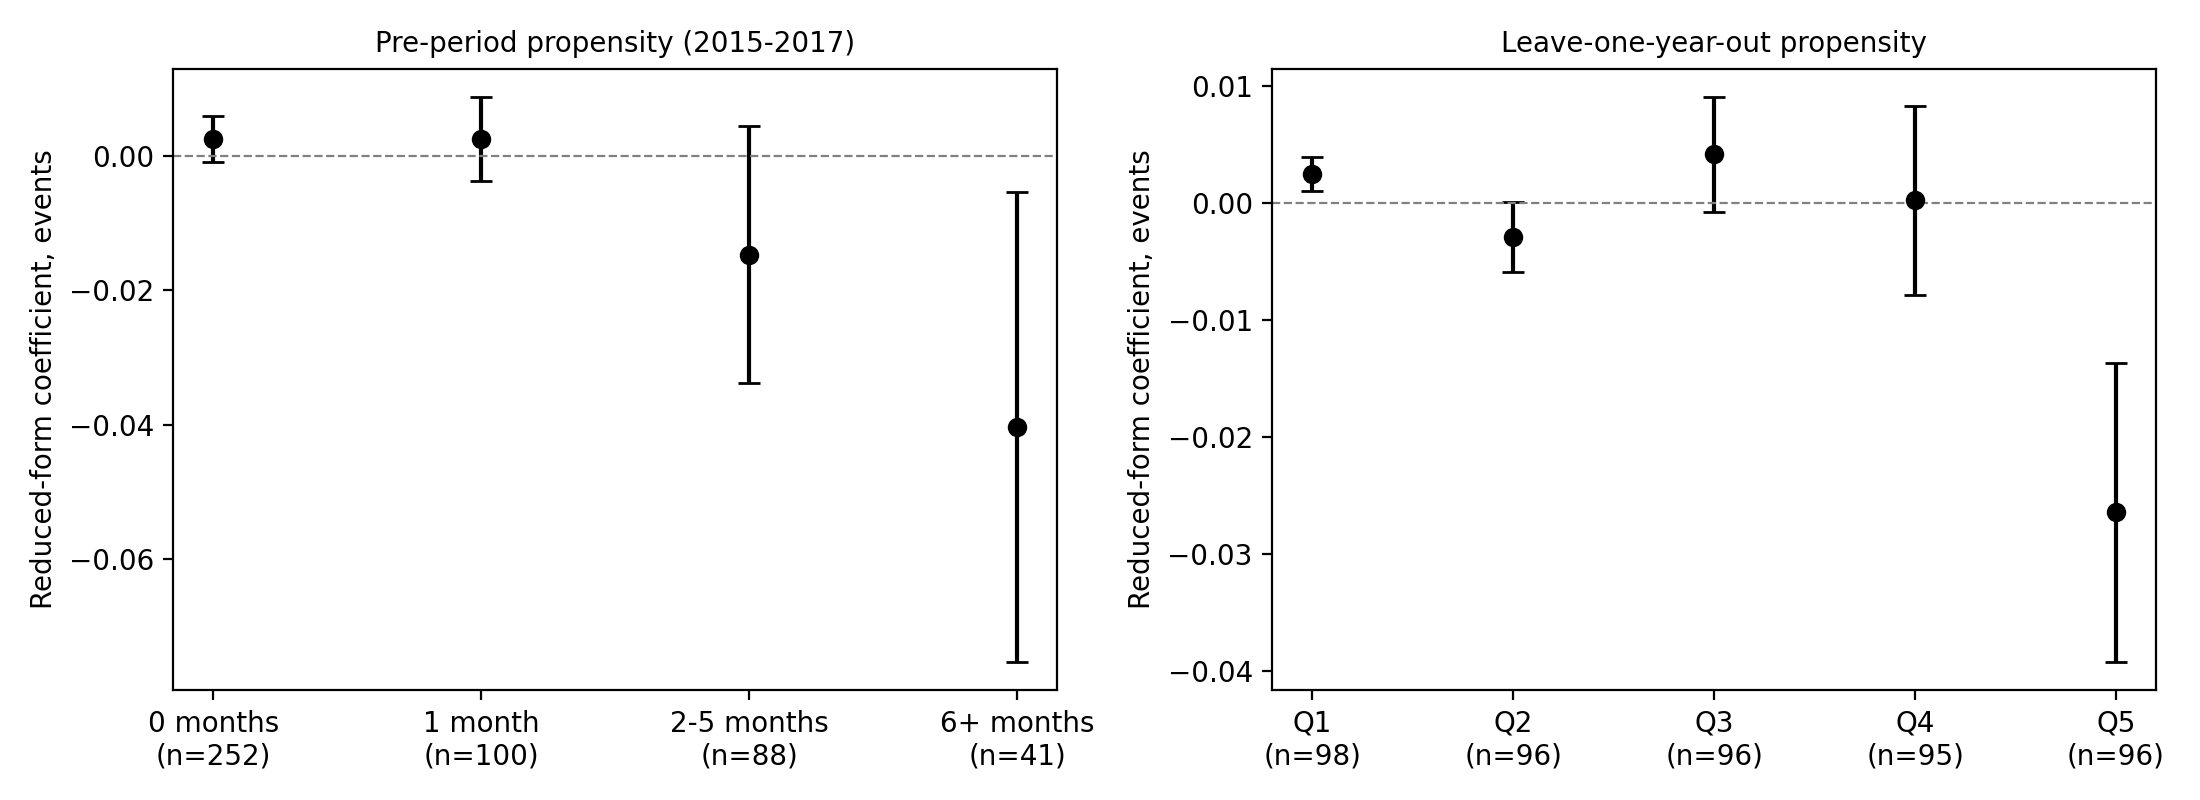
\includegraphics[width=\textwidth]{figures/conflict_propensity_bins.png}
\caption{Reduced-form effect of upwind fire by prior conflict propensity. Each point is the coefficient on contemporaneous log upwind FRP, estimated separately for each group, with 95\% confidence intervals from province-clustered standard errors. Left: districts grouped by months with any event in 2015--2017, estimated on 2018--2025. Right: quintiles of leave-one-year-out conflict propensity, estimated on 2015--2025.}
\label{fig:propensity}
\end{figure}

\begin{table}[H]
\centering
\caption{Robustness of the reduced form, all events, conflict-active districts}
\label{tab:robust}
\footnotesize
\begin{tabular}{lccc}
\toprule
Specification & Districts & Coefficient on $\text{logZ}_{dt}$ & $p$-value \\
\midrule
Baseline & 85 & $-0.0261$ & 0.002 \\
\addlinespace
\multicolumn{4}{l}{\emph{Regional seasonality and weather}} \\
\quad + one-month lead of the instrument & 85 & $-0.0256$ & 0.001 \\
\quad\quad lead coefficient & & $-0.0002$ & 0.985 \\
\quad + precipitation and temperature (and lags) & 85 & $-0.0262$ & 0.002 \\
\quad + weather and province $\times$ calendar-month FE & 85 & $-0.0262$ & 0.013 \\
\quad + province $\times$ year-month FE & 85 & $-0.0277$ & 0.190 \\
\addlinespace
\multicolumn{4}{l}{\emph{Measurement and sample}} \\
\quad Instrument excludes fires inside the district & 85 & $-0.0294$ & 0.004 \\
\quad 2018--2025 only & 85 & $-0.0362$ & 0.003 \\
\quad 2018--2025, districts re-selected on 2018--2025 & 117 & $-0.0303$ & 0.002 \\
\quad Excluding Papua and Papua Barat & 70 & $-0.0200$ & 0.041 \\
\addlinespace
\multicolumn{4}{l}{\emph{Placebo}} \\
\quad Upwind fire of a random district $\geq 500$\,km away & 85 & $+0.0023$ & 0.802 \\
\bottomrule
\end{tabular}
\begin{minipage}{0.95\textwidth}
\vspace{4pt}
\footnotesize \emph{Notes:} Each row reports the coefficient on contemporaneous log upwind FRP in Eq.~\eqref{eq:rf} with all events as the outcome, modified as indicated. District and year-month fixed effects in all rows; standard errors clustered by province.
\end{minipage}
\end{table}

Table~\ref{tab:robust} shows that the estimate is stable. Next month's upwind fire does not predict this month's conflict, so the instrument is not picking up regional seasonal trends. Weather controls leave the estimate unchanged, so it does not reflect drought, and excluding fires inside the district leaves it unchanged, so it does not reflect local burning. It is larger in 2018--2025, when ACLED's coverage is better, and a placebo built from a distant district's upwind fire has no effect. Two checks are weaker. Province-by-year-month fixed effects leave the point estimate intact but remove most of the variation ($p=0.19$), so province-wide shocks cannot be ruled out. And excluding Papua, the site of an active insurgency, shrinks the estimate to $-0.020$ ($p=0.041$).

\section{Mechanisms}
\label{sec:mechanisms}

If haze kept people indoors, protests should fall most; if it diverted security forces to fire response, events carried out by state forces should; if it crowded out reporting, low-salience and imprecisely recorded events should. Poisson estimates, which give comparable proportional effects, favor the second. Events carried out by state forces fall by 6.3\% per log point ($p<0.001$), about five times as much as peaceful protests ($-1.4\%$, $p=0.017$), which dominate the decline in levels only because they are the most common event type. Fatal events, the least likely to go unreported, fall by 5.2\% ($p=0.007$), and imprecisely located or dated events do not fall at all ($p=0.96$), the opposite of what a reporting explanation predicts. Conflict is not merely postponed: the four-month cumulative effect is larger than the contemporaneous one.

Fire task forces are organized by province, so fires in a district's own province draw on its security forces, while fires in another province reach it only as smoke. I split upwind FRP into these two components, which are only weakly correlated (0.23), and estimate the reduced form with both (Table~\ref{tab:province}).

\begin{table}[H]
\centering
\caption{Same-province and other-province upwind fire (conflict-active districts, PPML)}
\label{tab:province}
\footnotesize
\begin{tabular}{lccc}
\toprule
 & Same-province & Other-province & Equality \\
Outcome & coef. (SE) & coef. (SE) & $p$-value \\
\midrule
All events & $-0.004$ (0.008) & $-0.013^{**}$ (0.005) & 0.347 \\
Peaceful protests & $-0.003$ (0.007) & $-0.018^{***}$ (0.005) & 0.078 \\
Carried out by state forces & $-0.045^{***}$ (0.017) & $-0.038$ (0.043) & 0.880 \\
Violence against civilians & $-0.064^{***}$ (0.016) & $-0.028$ (0.035) & 0.363 \\
VAC by state forces & $-0.068^{***}$ (0.017) & $-0.048$ (0.047) & 0.702 \\
Non-state violence & $-0.001$ (0.025) & $+0.005$ (0.019) & 0.875 \\
\bottomrule
\end{tabular}
\begin{minipage}{0.95\textwidth}
\vspace{4pt}
\footnotesize \emph{Notes:} Poisson reduced form with log same-province and log other-province upwind FRP and the one-month lag of each; coefficients on the contemporaneous components. ``Equality'' tests that the two coefficients are equal. District and year-month fixed effects; standard errors clustered by province. $^{***}p<0.01$, $^{**}p<0.05$, $^{*}p<0.1$.
\end{minipage}
\end{table}

Protests fall with other-province fire ($-1.8\%$, $p=0.001$) but not with same-province fire, so their decline is best explained by smoke itself. Events carried out by state forces fall significantly only with same-province fire ($-4.5\%$, $p=0.009$), consistent with security forces being diverted to fire response, although the imprecise other-province estimate means equal effects cannot be rejected. Both patterns hold outside Papua. Same-province fires are also closer on average, so the contrast is partly between near and far fires.

Finally, instrumenting MERRA-2 reanalysis PM2.5 \citep{gelaro2017merra} with upwind fire gives a strong first stage (effective $F=25.7$) and a negative effect of pollution on conflict (Anderson--Rubin $p=0.004$). But satellite-observed aerosols do not respond detectably to upwind fire, plausibly because clouds and smoke remove the haziest days from the satellite record, so the pollution channel is suggestive rather than confirmed.

\section{Conclusion}

Wind-borne fire exposure reduces conflict in Indonesia by a small percentage, through two channels: smoke discourages protest, and fire response plausibly diverts security forces from the operations in which they come into violent contact with civilians. The negative sign contrasts with evidence that climate shocks and pollution increase conflict and crime, plausibly because haze is an acute shock that acts through logistics rather than income, and because the events studied here are collective or organized acts that depend on coordination and on the capacity of the security forces. Records of security-force deployments, daily pollution data, and replication in other fire-prone countries would sharpen these conclusions.

\bibliographystyle{plainnat}
\bibliography{references}

\end{document}
